\documentclass[../cheatSheetAlgoritmi.tex]{subfiles}
\begin{document}

\section{Esami anni passati}
\subsection{Esame 22/08/2019}
\textbf{Albero binario 1-bilanciato} \\
Un albero binario è \emph{1-bilanciato} se e solo se, per ogni nodo dell'albero, la differenza fra l'altezza del suo sottoalberodestro e l'altezza del suo sottoalbero sinistro è al più 1. \\
Scrivere un algoritmo che prenda in input un’altezza \emph{h} e restituisca il numero di alberi binari 1-bilanciati strutturalmente diversi di altezza \emph{h}. \\
Discutere informalmente la correttezza dell’algoritmo e calcolare la sua complessità computazionale. \\
Nella figura sotto, l’albero di sinistra è \emph{1-bilanciato}, l'albero di destra no, in quanto il sottoalbero sinistro di \emph{t} ha altezza 0 e il sottoalbero destro ditha altezza 2; la differenza è quindi maggiore di 1.
\begin{center}
	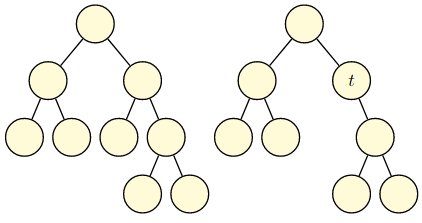
\includegraphics{../img/esame_22082019}
\end{center}
\textbf{Soluzione}  \\
Il docente propone una soluzione molto efficiente basata su programmazione dinamica. \\
La definizione ricorsiva del problema è la seguente: \\ 
Sia $DP[h]$ il numero di alberi 1-bilanciati di altezza \emph{h}. Allora possono presentarsi i seguenti casi:
\begin{itemize}
	\item Se $h = 0$, stiamo parlando di un nodo singolo, con altezza 0; esiste un solo albero di questo tipo.
	\item Se $h = 1$, esistono tre casi possibili: una radice con un solo figlio destro, una radice con un solo figlio sinistro, una radice con entrambi i figli.
	\item Se $h > 1$, possono darsi tre casi: 
		\begin{itemize}
			\item Il figlio destro è una radice di un sottoalbero di altezza $h - 1$, mentre il figlio sinistro è radice di un sottoalbero di altezza $h - 2$;
			\item Il figlio sinistro è una radice di un sottoalbero di altezza $h - 1$, mentre il figlio destro è radice di un sottoalbero di altezza $h - 2$;
			\item Sia il figlio destro che sinistro sono radice di un sottoalbero di altezza $h - 1$.
		\end{itemize}
		In tutti questi casi, i sottoalberi destro e sinistro devono essere 1-bilanciati essi stessi (come era intuibile)
\end{itemize}
È quindi possibile esprimere la formula ricorsiva in questo modo: 
\begin{equation*}
  	DP[h] =\begin{cases}
    	1 & \text{$h = 0$}\\
    	3 & \text{$h = 1$}\\
    	2 \cdot DP[h - 1] \cdot DP[h - 2]  + DP[h - 1] \cdot DP[h - 1] & \text{$h > 1$}
  	\end{cases}
\end{equation*}
Una volta ricavata questa (la grande difficoltà di questo esercizio è proprio la formula ricorsiva, dato che non è semplice metterci nella condizione di considerare, data una radice, i possibili figli destri e sinistri) è possibile tradurla in codice come segue grazie a programmazione dinamica:
singola volta.
\begin{lstlisting}[ caption = Alberi 1-bilanciati strutturalmente diversi]
int balanced(int h)
	int[] DP = new int[0...h]
	DP[0] = 1
	DP[1] = 3
	for i = 2 to h do
		DP[h] = $2 \cdot DP[i - 1] \cdot DP[i - 2] + DP[i - 1] \cdot DP[i - 1]$
	return DP[h]
\end{lstlisting}
\textbf{Considerazioni} \\
La complessità è lineare nel numero di operazioni di lettura/scrittura del vettore DP; tenete conto tuttavia che il numero di alberi cresce più che esponenzialmente, quindi le operazioni di moltiplicazione e somma non hanno costo lineare in \emph{h}.
\newpage
\end{document}
